% Chapter 1

\chapter{绪论}

\section{概述}
  计算机在对一个平面多边形进行栅格化时,一般需要将其切分为多个三角形的并,之后对每个小三角形依次渲染,最终合并出原多边形。在切分出的三角形中,具有两个极小锐角的细长三角形被称为“sliver triangles”\upcite{edelsbrunner2000smoothing},具有一些不利于后续计算的特性。
  细长三角形由于具有极小的锐角,从三角形的末端开始存在较长一段区域宽度极小,渲染时不足一个像素,因此会由于精度原因丢失内容。
  另外,细长三角形由于长度过长,会导致多边形内较多的出现距离较近的点属于不同三角形,而距离较远的两个点却属于同一三角形的问题。
  因此,在设计多边形栅格化的算法时,常常需要在做到高效的同时避免细长三角形的大量产生。

  本文设计并实现了两种近似算法,可在不添加新顶点的情况下快速将任意形状带孔凹多边形划分成数个互不重合的三角形,能正确处理多种复杂情况,且产生的细长三角形数目较少,便于后续处理。
\section{研究现状}

平面多边形三角化作为计算机图形学的基础课题,在计算机图形处理,有限元网格自动生成\upcite{brown1981non},计算机图像处理,三维立体造型\upcite{yamaguchi1983solid}等多个方面有着广泛的应用\upcite{陈向平1989统一于}。当下对平面多边形三角化的研究较为成熟,有着较多的相关研究。
陈向平\upcite{陈向平1989统一于}提出了一种基于耳切法的三角剖分算法实现,可以计算出任意平面多边形的一种合法三角划分结果。
闵卫东讨论\upcite{闵卫东1995二维任意域内点集的}并给出\upcite{闵卫东1995二维任意域内点集的Delaunay三角划分生成算法}了一种生成二维任意域内点集三角剖分的算法,并讨论了本问题的理论复杂度下界。
马小虎等人\upcite{马小虎1999基于凹凸顶点判定的简单多边形}提出了一种经改进的耳切法三角剖分实现,给出了一种在\(O(n^3)\)的时间复杂度内计算平面多边形Delaunay三角划分的算法。

杨军\upcite{杨军2016格网划分的}提出了一种基于格网划分法的三角剖分实现,对逐点插入算法进行了优化,提高了该算法在构建三角网时的运行效率。
近期的研究则以对已有的三角划分算法应用为主,在GIS\upcite{刘学军2001三角网数字地面模型的理论},医学图像\upcite{秦绪佳2002医学图像三维重建模型的剖切与立体视窗剪裁},地球物理学\upcite{王永奎2022基于三角网格模型剖分的高斯束正演数值模拟},工业制造\upcite{丁植2022基于},机器视觉\upcite{连静2023复杂交通环境下基于关键目标的视觉},计算机图形学等方面有着较多研究成果。


三角剖分(triangulation):假设在平面有一点集V,三角形s是由点集中的点作为端点的非退化三角形,S为s的集合。则该点集V的一个三角剖分T=(V,S)是一个平面图,满足以下条件:
\begin{itemize}
  \item 平面图中的任意两个三角形交集面积为0
  \item 平面图中所有三角形的并集是点集V的凸包
\end{itemize}

Ear Clipping(耳切法)\upcite{eberly2008triangulation}是一种较为简易的多边形三角化算法,其思路简单易懂,但缺点是可能会产生较多的细长三角形。原理为不断在多边形内寻找可被切除\footnote[1]{当一个三角形内部不包含其他顶点且该三角形属于原多边形一部分时认为其可切除}的连续三个顶点构成的三角形。对于任意多边形,至少存在两个可被切除的三角形。轮流切除所有的三角形后算法结束。朴素情况下该算法的复杂度约为\(O(n^2)\)。

\begin{figure}[htbp]
  \centering
  \begin{minipage}{0.4\textwidth}
      \centering
      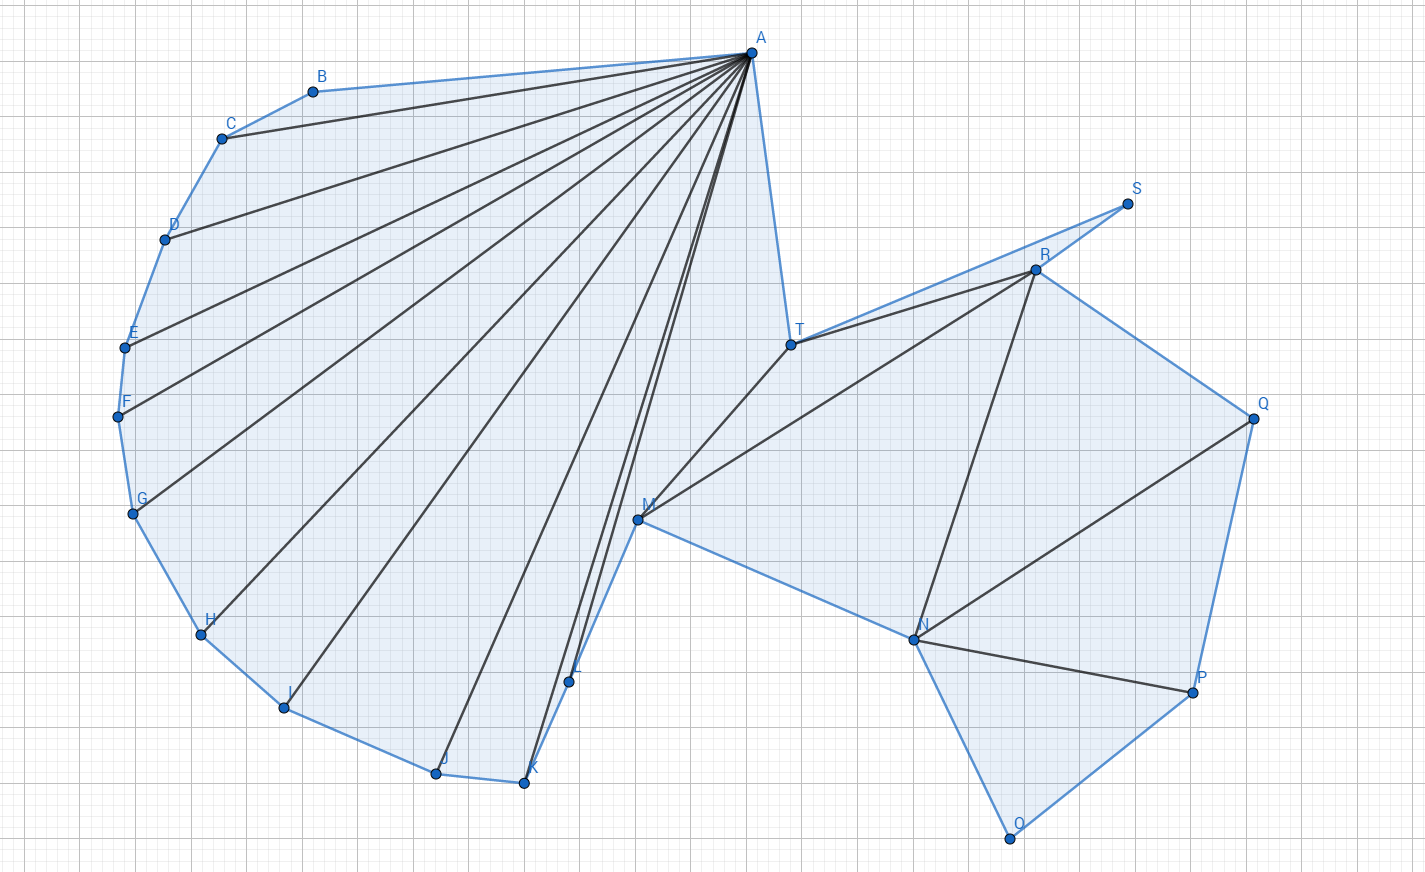
\includegraphics[width=\textwidth]
      {figures/ear clipping.png}
      \caption{耳切法的典型结果}
  \end{minipage}
  \begin{minipage}{0.4\textwidth}
      \centering
      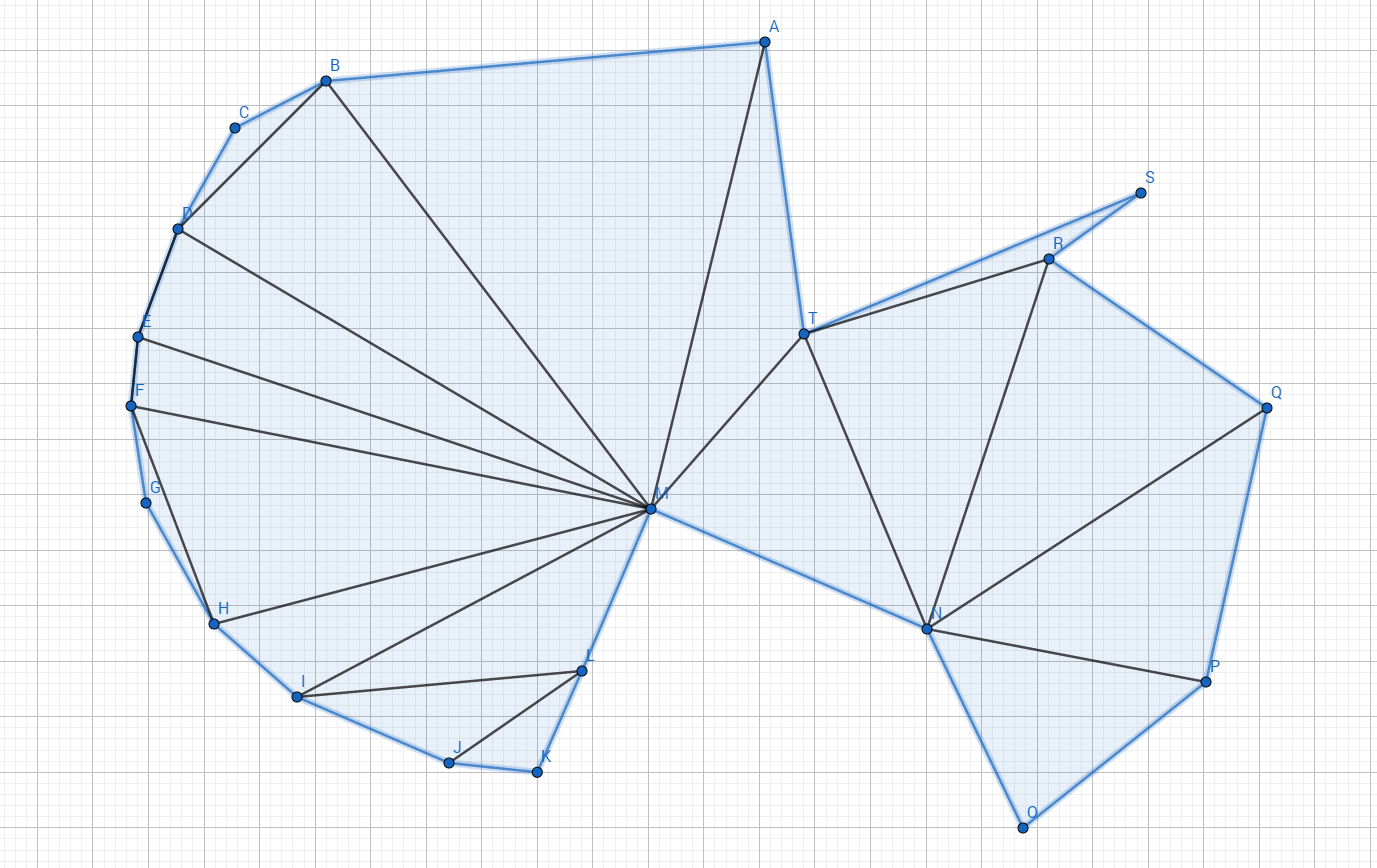
\includegraphics[width=\textwidth]
      {figures/better.png}
      \caption{相对更好的一种解}
  \end{minipage}
\end{figure}

Delaunay triangulation\upcite{lee1980two}算法则会生成一组相对更加优秀的解,其满足形成的三角形中最小角尽可能大。但该算法只适用于凸多边形的划分。虽然计算得出的解在处理后也可用于凹多边形划分,但该划分结果可能会产生新的顶点,导致最终的三角形个数增加。Delaunay三角划分有数种实现方式,其中较为常用的算法如Bowyer-Watson算法,其原理是维护一个合法的Delaunay三角划分,每次向点集中加入新点,并修改新增点附近的三角划分规则。其复杂度为\(O(n^2)\)。或者也可以采用分治法,将点集划分为两部分并合并生成的Delaunay三角划分,其时间复杂度为\(O(n*\log_2n)\)。
当下存在一些改进的Delaunay三角网生成算法,可以将算法的运行效率进一步提高,使算法运行时间的增长更趋近于线性\upcite{尤磊2022自适应二分的并行Delaunay三角网生长算法}。

可以看出,上面的两种三角化算法各有优劣。

耳切法逻辑简单易懂,能够处理任意形状的多边形,对于多边形形态这一方面具有最大的兼容性。
但其在产生的多边形形态上缺少控制,贪心的选择能够从当前多边形直接切除的一个三角形,未考虑切除多边形的形态是否较优。

Delaunay三角划分的实现相对来说更加复杂,精度最高,但是只能对凸多边形产生正确的结果。对凹多边形或带孔多边形进行处理时,无法考虑到多边形内已有的边,会产生与之冲突的剖分结果,导致需要在冲突处新增顶点,将之前的切分线分成两段,才能处理一般情况下的多边形。

\section{方法概述}

定义\(N_i\) 为二维平面上的点,\(N_{ix},N_{iy}\) 分别为该点的横纵坐标;

定义有序集合\(S:N_0,N_1,\cdots,N_{n-1}\)表示有n个节点的无孔洞简单多边形,对任意\(i\in [0,n-1] \)满足\(N_i,N_{(i+1) \bmod n}\)之间存在一条连边。

定义有序集合\(T:S_0,S_1,\cdots,S_{n-1}\)表示有n段边界的有孔洞简单多边形,其中\(S_0\)表示多边形的外边界,其余则表示多边形中的孔洞。

本文分別通过将多边形逐步细分为凸多边形和向多边形顶点集中加入约束边两种思路实现了任意凸多边形的三角化。
在对多边形进行逐步细分的过程中,本文根据待处理多边形的性质进行分类讨论,并逐步消除多边形中的自交,孔洞,凹点等复杂特征,最终在尽可能少破坏解的同时将原多边形细分为数个凸多边形,以快速计算出其唯一Delaunay三角划分。
在向多边形顶点集加入约束边的过程中,本文提出了一种通过对角线交换消除候选边冲突的思路,可以快速处理约束边所产生的冲突。
\section{章节安排}
本文将分为五个章节展开论述与研究。
第一章为本文的绪论。首先对本课题的研究背景与目的展开介绍,其次分析当前采用的数种三角剖分算法所具有的特点,优势及不足,并简要介绍当前基础三角剖分算法的原理。接下来介绍了本文所用到的概念定义与文章章节安排。

第二章为细分算法的流程介绍及证明。本章从复杂多边形开始逐步介绍了本文中对多边形进行细分的算法流程,证明了其复杂度及正确性。
本章还介绍了细分算法中所采用的局部优化及创新点。

第三章为分治算法的流程介绍及证明。本章介绍了基于点集Delaunay三角网生成待约束三角网,并根据约束三角网生成三角剖分结果的过程。

第四章为实验部分的介绍。本文通过手工构造的实验数据验证了上述算法的效果,并通过随机生成的大规模图像数据将本文中算法与数种现有算法进行对比,讨论了不同优化点所产生的差异。

第五章为总结与展望。我们总结了本文中算法的核心特点,并提出了数个算法中仍待改进的不足之处。

% 与Word等所见即所得编辑工具不同,使用 \LaTeX 工具排版可以将写作与排版过程分离,写作者只需要关心文字的部分,而剩下的排版工作全部交给工具自动完成。

% \section{格式要求}
% 正文宋体小四,正文行间距固定为23磅。

% 通过空一行(两次回车)实现段落换行,仅仅是回车并不会产生新的段落。 \par

% 也可以通过 \verb|\par| 命令来新起一段。

% \section{各节一级标题}
% 我是内容

% \subsection{各节二级标题}
% 你是内容

% \subsubsection{各节三级标题}
% 他是内容

% \section{字体字号}
% {\songti \bfseries 宋体加粗} {\textbf{English}}

% {\songti \itshape 宋体斜体} {\textit{English}}

% {\songti \bfseries \itshape 宋体粗斜体} {\textbf{\textit{English}}}

% \section{编译}
% 本模板必须使用XeLaTeX + BibTeX编译,否则会直接报错。 本模板支持多个平台,结合sublime/vscode/overleaf都可以使用。